\documentclass[pdftex,12pt,a4paper]{article}

% Это пустая болванка для написания небольшого документа

\usepackage{etex} % расширение классического tex

% для русского языка...
\usepackage{cmap} % для поиска русских слов в pdf
\usepackage[X2,T2A]{fontenc} % кодирование шрифтов в pdf
\usepackage[utf8]{inputenc} % задание utf8 кодировки исходного tex файла
\usepackage[british,russian]{babel} % выбор языка для документа

\usepackage{verbatim} % для многострочных комментариев
\usepackage{makeidx} % для создания предметных указателей
\usepackage{indentfirst} % установка отступа в первом абзаце главы

\usepackage{amsmath,amsfonts,amssymb,amsthm} % символы и формульные окружения от AMS
\usepackage{bm, bbm} % шрифты

\usepackage{dcolumn} % центрирование по разделителю для apsrtable
\usepackage{longtable} % таблицы на несколько страниц
\usepackage{booktabs} % красивые таблицы
% заповеди из документации: 
% 1. Не используйте вертикальные линни
% 2. Не используйте двойные линии
% 3. Единицы измерения - в шапку таблицы
% 4. Не сокращайте .1 вместо 0.1
% 5. Повторяющееся значение повторяйте, а не говорите "то же"

% создание гиперссылок в pdf
\usepackage[pdftex,unicode,colorlinks=true,urlcolor=blue,hyperindex,breaklinks]{hyperref} 

\usepackage{microtype} % свешиваем пунктуацию 
\usepackage{textcomp}  % Чтобы в формулах можно было русские буквы писать через \text{}

\usepackage{enumitem} % дополнительные плюшки для списков
%  например \begin{enumerate}[resume] позволяет продолжить нумерацию в новом списке

\usepackage[pdftex]{graphicx} % для вставки графики 
\usepackage{subfigure} % для создания нескольких рисунков внутри одного

\usepackage{tikz,pgfplots} % язык для рисования графики из latex'a
\usetikzlibrary{trees} % tikz-прибамбас для рисовки деревьев
\usepackage{tikz-qtree} % альтернативный tikz-прибамбас для рисовки деревьев
\usetikzlibrary{arrows} % tikz-прибамбас для рисовки стрелочек подлиннее

\usepackage{todonotes} % для вставки в документ заметок о том, что осталось сделать
% \todo{Здесь надо коэффициенты исправить}
% \missingfigure{Здесь будет Последний день Помпеи}
% \listoftodos --- печатает все поставленные \todo'шки

% Вложение файлов в готовый pdf 
\usepackage{embedfile} % пакет для включения других файлов
\embedfile[desc={Main tex file}]{\jobname.tex} % Включение данного файла в готовый pdf
%\embedfile[desc={title_bor}]{my_file.zip} % включение произвольного файла

%%%%%%%%%%%%%%%%%%%%%%%%%%%%%%%%%%%%%%%%%%%%%%%%%%%%%%%%%%%%%
%%%%%%%% УРААААААААААААААААААААААААААААААААААААААААААААААААА
%%%%%%%% Начинается документ...

% размер листа бумаги
\usepackage[paper=a4paper,top=12.5mm, bottom=12.5mm,left=12.5mm,right=12.5mm,includefoot]{geometry}


\title{B10 в КОГОАУ КЭПЛ}
\author{Борис Демешев, \href{mailto:boris.demeshev@gmail.com}{boris.demeshev@gmail.com}}
\date{25 февраля 2013}
%\institute{НИУ ВШЭ}


\begin{document}
\begin{center}
{\Large B10 в КОГОАУ КЭПЛ\footnote{Борис Демешев, \href{mailto:boris.demeshev@gmail.com}{boris.demeshev@gmail.com}, 25 февраля 2013}}
\end{center}
%\maketitle % помещаем сюда заголовок
% \parindent=0 pt % ставлю отступ красной строки = 0

\textbf{Каждый может посадить дерево!}

\begin{enumerate}

\item Две фабрики выпускают одинаковые стекла для автомобильных фар. Первая фабрика выпускает 45\% этих стекол, вторая --- 55\%. Первая фабрика выпускает 3\% бракованных стекол, а вторая --- 1\%. Найдите вероятность того, что случайно купленное в магазине стекло окажется бракованным.

\item Всем пациентам с подозрением на гепатит делают анализ крови. Если анализ выявляет гепатит, то результат анализа называется положительным. У больных гепатитом пациентов анализ даёт положительный результат с вероятностью 0,9. Если пациент не болен гепатитом, то анализ может дать ложный положительный результат с вероятностью 0,01. Известно, что 5\% пациентов, поступающих с подозрением на гепатит, действительно больны гепатитом. Найдите вероятность того, что результат анализа у пациента, поступившего в клинику с подозрением на гепатит, будет положительным.

\item Ковбой Джон попадает в муху на стене с вероятностью 0,9, если стреляет из пристрелянного револьвера. Если Джон стреляет из непристрелянного револьвера, то он попадает в муху с вероятностью 0,2. На столе лежит 10 револьверов, из них только 4 пристрелянные. Ковбой Джон видит на стене муху, наудачу хватает первый попавшийся револьвер и стреляет в муху. Найдите вероятность того, что Джон промахнётся.
\end{enumerate}

\textbf{Табличка с количествами\ldots}

\begin{enumerate}

\item Вероятность того, что новый электрический чайник прослужит больше года, равна 0,97. Вероятность того, что он прослужит больше двух лет, равна 0,89. Найдите вероятность того, что он прослужит меньше двух лет, но больше года.

\item В торговом центре два одинаковых автомата продают кофе. Вероятность того, что к концу дня в автомате закончится кофе, равна 0,3. Вероятность того, что кофе закончится в обоих автоматах, равна 0,12. Найдите вероятность того, что к концу дня кофе останется в обоих автоматах.

\item В магазине стоят два платёжных автомата. Каждый из них может быть неисправен с вероятностью 0,05 независимо от другого автомата. Найдите вероятность того, что хотя бы один автомат исправен.

\item Агрофирма закупает куриные яйца в двух домашних хозяйствах. 40\% яиц из первого хозяйства — яйца высшей категории, а из второго хозяйства — 20\% яиц высшей категории. Всего высшую категорию получает 35\% яиц. Найдите вероятность того, что яйцо, купленное у этой агрофирмы, окажется из первого хозяйства.
\end{enumerate}


\begin{comment}
\begin{center}
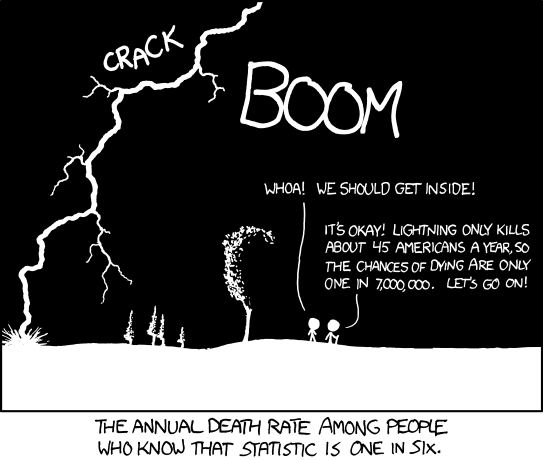
\includegraphics[height=60mm]{conditional_risk.png}
\end{center}

--- Ого! Молния! Лучше бы вернуться домой \\
--- Всё нормально! Молния убивает в среднем одного человека из семи миллионов. 
\vspace{5pt}

{\footnotesize Среди тех, кто знает эти вероятности, смертность равна одной шестой}
\end{comment}

\textbf{В каком порядке тянуть жребий?}
\begin{enumerate}

\item На семинар приехали 3 ученых из Норвегии, 3 из России и 4 из Испании. Порядок докладов определяется жеребьёвкой. Найдите вероятность того, что восьмым окажется доклад ученого из России.

\item Научная конференция проводится в 5 дней. Всего запланировано 75 докладов — первые три дня по 17 докладов, остальные распределены поровну между четвертым и пятым днями. Порядок докладов определяется жеребьёвкой. Какова вероятность, что доклад профессора М. окажется запланированным на последний день конференции?

\item Перед началом первого тура чемпионата по бадминтону участников разбивают на игровые пары случайным образом с помощью жребия. Всего в чемпионате участвует 26 бадминтонистов, среди которых 10 участников из России, в том числе Руслан Орлов. Найдите вероятность того, что в первом туре Руслан Орлов будет играть с каким-либо бадминтонистом из России?

\item В классе 26 человек, среди них два близнеца  — Андрей и Сергей. Класс случайным образом делят на две группы по 13 человек в каждой. Найдите вероятность того, что Андрей и Сергей окажутся в одной группе.

\item Колода из 36 карт хорошо перемешана. В любой момент можно сказать <<Стоп! Следующая карта --- пиковой масти>>. Если это окажется правдой, то Вы выигрываете 100 рублей. Какова оптимальная стратегия? Какова вероятность выигрыша при оптимальной стратегии? 
\end{enumerate}



\textbf{Два измерения --- непрерывный случай}

\begin{enumerate}
\item В случайном эксперименте бросают две игральные кости. Найдите вероятность того, что в сумме выпадет 8 очков. Результат округлите до сотых.
\item Аня и Боря независимо друг от друга приходят на лыжах на Южный Полюс между 12:00 и 13:00. Каждый из них ждёт 10 минут, а потом уезжает. Какова вероятность того, что они встретятся?
\end{enumerate}


\textbf{Биномиальная случайная величина}

\begin{enumerate}
\item В Волшебной стране бывает два типа погоды: хорошая и отличная, причём погода, установившись утром, держится неизменной весь день. Известно, что с вероятностью 0,8 погода завтра будет такой же, как и сегодня. Сегодня 3 июля, погода в Волшебной стране хорошая. Найдите вероятность того, что 6 июля в Волшебной стране будет отличная погода.

\item Вася стреляет по мишени 4 раза. Каждый раз независимо от других он попадает с вероятностью 0.7. Какова вероятность того, что он попадёт ровно 3 раза? Ровно 2 раза?
\end{enumerate}

\vspace{50pt}

\begin{flushleft}
Я очнулся в цветах, а вокруг уже ночь,  \\
Лепестков облетевших одежда полна.  \\
Вдоль ручья побреду я куда-нибудь прочь,  \\
Где ни птиц, ни людей, только в небе Луна.  
\end{flushleft}


\begin{flushright}
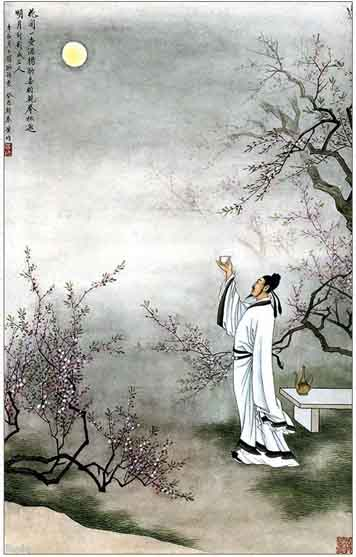
\includegraphics[height=50mm]{libo_moon.jpg}

Ли Бо 
\end{flushright}





\end{document}
